\paragraph{QuizziPedia::Front-End::Controllers::QuestionsManagementController}
\begin{figure} [ht]
	\centering
	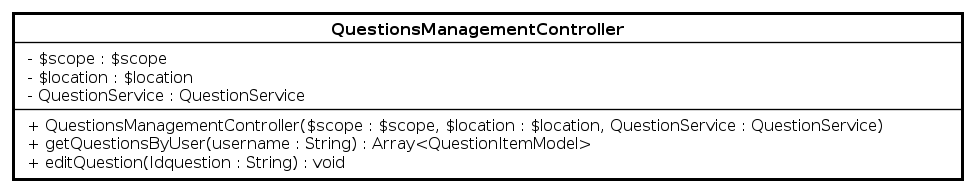
\includegraphics[scale=0.80]{UML/Classi/Front-End/QuizziPedia_Front-end_Controller_QuestionsManagementController.png}
	\caption{QuizziPedia::Front-End::Controllers::QuestionsManagementController}
\end{figure} \FloatBarrier
\begin{itemize}
	\item \textbf{Descrizione}: questa classe permette di gestire le domande create dall'utente e di crearne di nuove;
	\item \textbf{Utilizzo}: fornisce le funzionalità per richiedere al server le domande create dall'utente e mostrarle nella pagina dedicata. Inoltre permette di catturare gli eventi per modificare le domande esistenti e per crearne una di nuova; 
	\item \textbf{Relazione con altre classi}:
	\begin{itemize}
		\item \textit{IN} \texttt{QuestionsManagementModelView}: classe di tipo modelview la cui istanzazione è contenuta all'interno della variabile di ambiente \$scope di \textit{Angular.js\ped{G}}. All'interno di essa sono presenti le variabili e i metodi necessari per il \textit{Two-Way Data-Binding\ped{G}} tra la view \texttt{QuestionsManagementView} e il controller \texttt{QuestionsManagementController}; 
		\item \textit{IN} \texttt{QuestionService}: questa classe permette di ottenere domande esistenti e salvare nuove domande;
		\item \textit{IN} \texttt{QuestionsService}: questa classe permette di ottenere domande esistenti e salvare nuove domande.
	\end{itemize}
	\item \textbf{Attributi}:
	\begin{itemize}
		\item \texttt{-} \texttt{\$scope: \$scope} \\
		Campo dati contenente un riferimento all’oggetto \$scope creato da \textit{Angular\ped{G}}, viene utilizzato come mezzo di comunicazione tra il controller e la view. Contiene gli oggetti che definiscono il model dell’applicazione;
		\item \texttt{-} \texttt{\$location: \$location} \\
		Campo dati contenente un riferimento al servizio creato da \textit{Angular\ped{G}} che permette di accedere alla barra degli indirizzi del \textit{browser\ped{G}}, i cambiamenti all’URL nella barra degli indirizzi si riflettono in questo oggetto e viceversa;
		\item \texttt{-} \texttt{QuestionService}\\
		Campo dati contenente un riferimento al servizio che si occupa della gestione delle informazioni legate alle domande.
	\end{itemize}
	\item \textbf{Metodi}:
	\begin{itemize}
		\item \texttt{+} \texttt{QuestionsManagementsController(\$scope: \$scope, \$location: \$location, QuestionService: QuestionService)} \\ 
		Metodo costruttore della classe; \\
		\textbf{Parametri}:
		\begin{itemize}
			\item \texttt{\$scope: \$scope} \\
			Parametro contenente un riferimento all’oggetto \$scope creato da \textit{Angular\ped{G}}. Viene utilizzato come mezzo di comunicazione tra il controller e la view. Contiene gli oggetti che definiscono il viewmodel e il model dell’applicazione;
			\item \texttt{\$location: \$location} \\
			Parametro contenente un riferimento al servizio creato da \textit{Angular\ped{G}} che permette di accedere alla barra degli indirizzi del \textit{browser\ped{G}}, i cambiamenti all’URL nella barra degli indirizzi si riflettono in questo oggetto e viceversa;
			\item \texttt{QuestionService: QuestionService} \\
			Parametro contenente un riferimento al servizio che si occupa della gestione delle informazioni legate alle domande;
		\end{itemize}
		\item \texttt{+} \texttt{getQuestionsByUser(username: String)} \\ 
		Metodo che acquisisce le domande create dall'utente attraverso il \texttt{QuestionService};\\
		\textbf{Parametri}:
		\begin{itemize}
			\item \texttt{username: String} \\
			Parametro di tipo \texttt{String} contenente l'username dell'utente;
		\end{itemize}
		\item \texttt{+} \texttt{editQuestion(idQuestion: String)} \\ 
		Metodo che gestisce l’evento click sul pulsante per modificare la domanda. Effettua il redirect alla pagina di modifica della domanda. \\
		\textbf{Parametri}:
		\begin{itemize}
			\item \texttt{idQuestion: username} \\
			Parametro di tipo \texttt{String} contenente l'id della domanda da modificare;
		\end{itemize}
	\end{itemize}
\end{itemize}

